\chapter{Background and related work}

\section{Background}
\label{sec:Background}
This section presents the required field knowledge to understand this thesis. It therefore starts with an explanation on how a light source behaves when it turns on and off rapidly and why this is preferable over other light saving strategies. It then follows up with an explanation of how produced light travels and reflects off of surfaces.

\subsection{Dimming of an LED}
In this thesis, an LED will be used to illuminate the environment which will cause reflections in the room. It's therefore important to understand how the light responds to different methods of adjusting the light output, as this directly influences power of the reflections.

In general, there are two methods of dimming (reducing the light output of) an LED: Analogue and digital. A light which is dimmed in an analogue manner has its total light output reduced by reducing the current flowing into the LED. This leads to a light which has a constant light output directly proportional to the current flowing into the LED. If we for example want a light to produce 25\% of its normal light output, we simply supply it with a quarter of the current. A graphical representation of analogue dimming is shown in Figure \ref{fig:PWM} and is marked as "average power".

Digital dimming works in another way. Instead of controlling the amount of current flowing into the LED, we control the amount of time current is allowed to flow into the LED. This can be achieved by turning the LED on and off rapidly. If we for example want to reduce the light output of an LED to 25\% with the help of digital dimming, then we would turn the light on at full strength for 25\% of the time, while turning it off for 75\%, with the help of a Pulse Width Modulated (PWM) signal. A graphical representation of digital dimming is shown in Figure \ref{fig:PWM}.

The resulting light produced by both types of dimming are indistinguishable for humans if the switching frequency is high enough. Both methods have the same apparent brightness and use the same amount of power. For photo diodes however, there is a clear difference. The analogue signal will show up as a constant, but weak signal. The digital signal shows up as a square wave with high peaks (when the light is on) and valleys (when the light is off). This becomes especially apparent if we want the system to work at only 1\% of it's original illumination level. The signal dimmed in an analogue manner will be nearly invisible as it is turned on constantly at 1\% of it's original power. This in contrast to the digital signal, which only shows up for 1\% of the time, but at maximum power, resulting in a shorter but much brighter peak. Because the 1\% time constrain is no problem for an electronic system, it was chosen to explore Dark Sensing with this dimming method.

%turning on and off pattern
There is however a limit to how much the energy consumption can be reduced with digital dimming, if we want to be able to observe the signal with a photo diode. When an LED is turned on, it does not produce light at maximum intensity instantly\cite{LED_on}. It first has a short "turn-on delay" where the light does not output any light, followed by a "rise time" where the light "slowly" powers up until it has reached it's desired intensity level. A graphical representation of this process can be seen in figure \ref{fig:LedResponse}. This limit on digital dimming forces a hard minimum to the amount of digital dimming the system can work with and therefore limits the amount of energy it can save.

\begin{figure}[]
	\subfigure[]{\label{fig:PWM}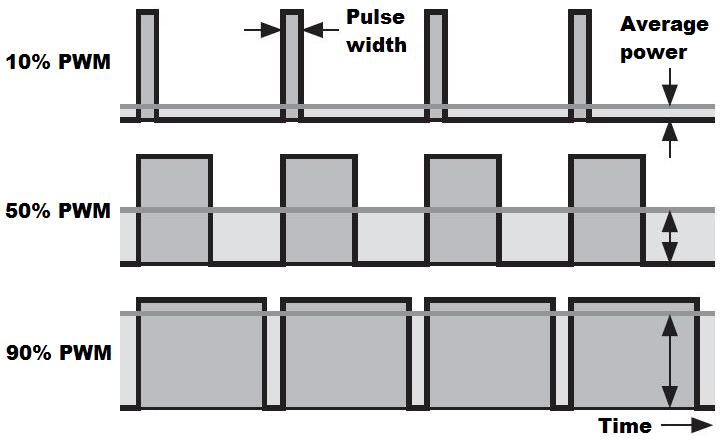
\includegraphics[width=60mm]{pics/PWM.png}}
	\subfigure[]{\label{fig:LedResponse}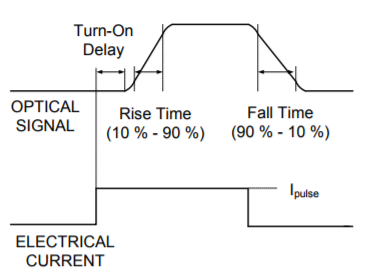
\includegraphics[width=60mm]{pics/LedResponse.png}}
	\caption{Figure (a) shows the difference between analogue and digital dimming, Figure (b) shows a realistic response of the light when a short electric pulse is applied\cite{LED_on}.\label{fig:LedOnTime}}
\end{figure}

\subsection{The Phong model}
\label{Model_explained}
When a light shines on a surface, some parts of the surface appear brighter than other parts. This is caused by three major factors:
\begin{itemize}[itemsep=-1ex,topsep=0pt]
	\item The light used to illuminate the wall and it's position relative to the wall.
	\item The surface of the wall itself.
	\item The position of the observer relative to the wall.
\end{itemize}
If all of these factors are known, then the complete pathing of the light can be approximated with the help of the Phong model. This section presents a simplified version of the Phong model which is used in chapter \ref{Model}. All used angles can be seen in Figure \ref{fig:model_overview}. The full model can be found in \cite{Advances_In_Optical_Communication}.

\begin{figure}
	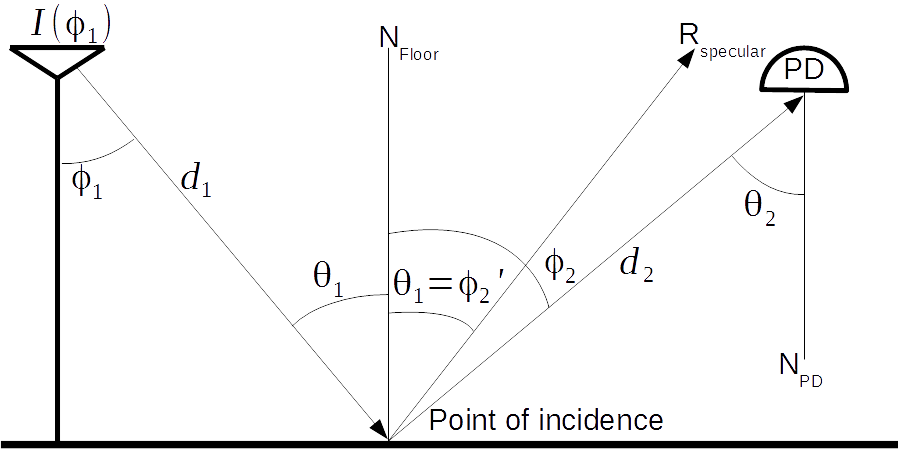
\includegraphics[width=\textwidth]{pics/single_light_post.png}
	\caption{Overview of angles, vectors and distances used in the model. It represents a street light illuminating the street (I). This light is then observed by a photo diode (PD), aimed at the ground. Note that $\phi$ always represents an exit angle and $\theta$ always represents an incidence angle.\label{fig:model_overview}}
\end{figure}

\subsubsection{Modelling an LED}
A light can be modelled if several parameters of the light are known, with the help of equation \ref{eq:I(phi)}. This formula describes how much light is leaving the light source at angle $\phi$ relative to the normal of the LED.
\begin{equation}
\label{eq:I(phi)}
I(\phi)=\Phi_{lum}\frac{\alpha+1}{2\pi}cos^\alpha(\phi_1)
\end{equation}
The equation consists of three parts. $\Phi_{lum}$ represents the total amount of light emitted in lumen by the LED. $cos^\alpha(\phi_1)$ represents the radiation pattern of the LED. $\alpha$ represents the order of Lambertian emission which describes the illumination pattern of the LED. If $\alpha$ is low (e.g. 1), then this equation represents a luminaire with a very wide spread of light, for example a street light. If $\alpha$ is high (e.g. 200+), then the light source is much more focused like a laser. An overview of $\alpha$ vales versus their angle is shown in Figure \ref{fig:cones_of_light}. $\frac{\alpha+1}{2\pi}$ is a normalisation factor that ensures that integrating equation \ref{eq:I(phi)} results in the total amount of light produced ($\Phi_{lum}$), as reshaping the cone of light with $\alpha$ would otherwise lead to a change in produced light. An example of a modelled light with $\alpha = 14.3$ and $\Phi_{lum} = 260lm$ can be seen in Figure \ref{fig:2lightcones}.

We can now take any light ray from the luminaire and calculate how much light hits a specific surface with the help of equation \ref{eq:E_hor}. This calculation also consists of three parts. The first part is the strength of the light ray calculated with equation \ref{eq:I(phi)}. The second part, $d$, represents the distance the light needs to travel before it hits the surface. The final variable, $\theta_1$, represents the incidence angle of the light ray on the surface.
\begin{equation}
\label{eq:E_hor}
E_{hor} = \frac{I(\phi_1)}{d^2} cos(\theta_1)
\end{equation}

%\begin{figure}
%	\centering     %%% not \center
%	\subfigure[]{\label{fig:Specs_a}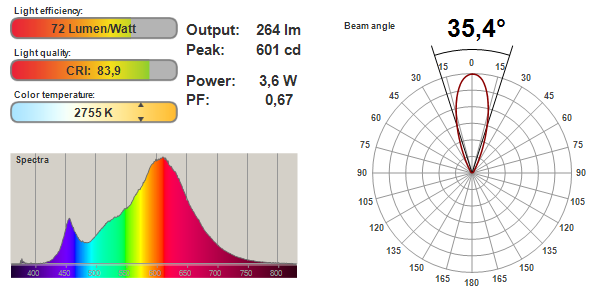
\includegraphics[width=68mm]{pics/LED_specs.png}}
%	\subfigure[Caclculated intensity pattern ]{\label{fig:Specs_b}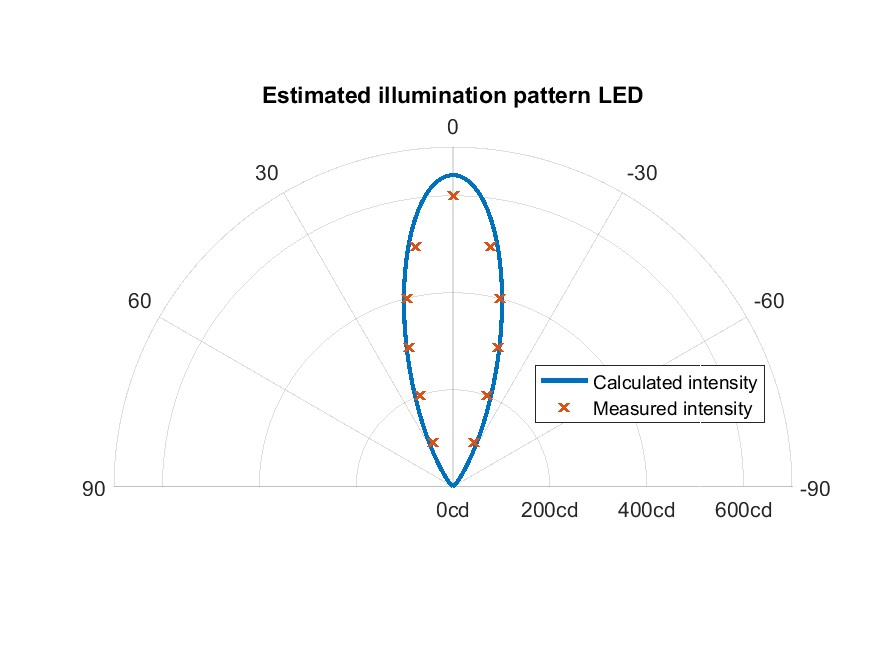
\includegraphics[width=52mm]{pics/polarplot_LED.png}}
%	\caption{Figure (a) shows measured specifications of an LED \cite{lamptest} where Figure (b) shows the estimated illumination pattern of the same LED with the described method.}
%\end{figure}

\begin{figure}
	\centering     %%% not \center
	\subfigure[]{\label{fig:cones_of_light}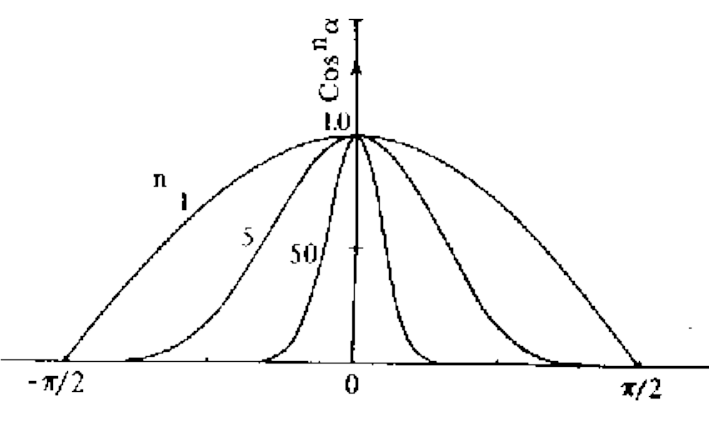
\includegraphics[width=60mm]{pics/cones_of_light.png}}
	\subfigure[]{\label{fig:2lightcones}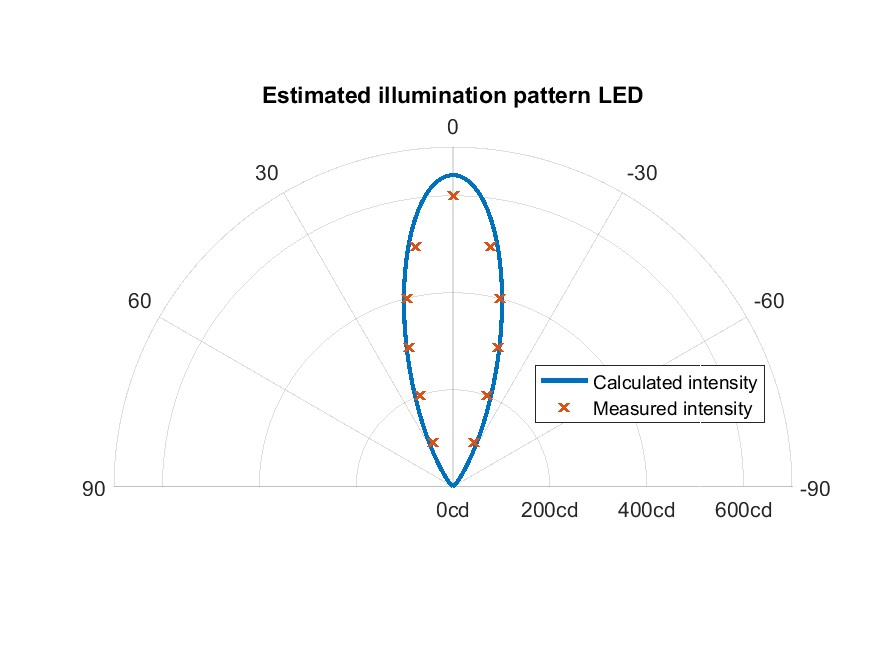
\includegraphics[width=60mm]{pics/polarplot_LED}}
%	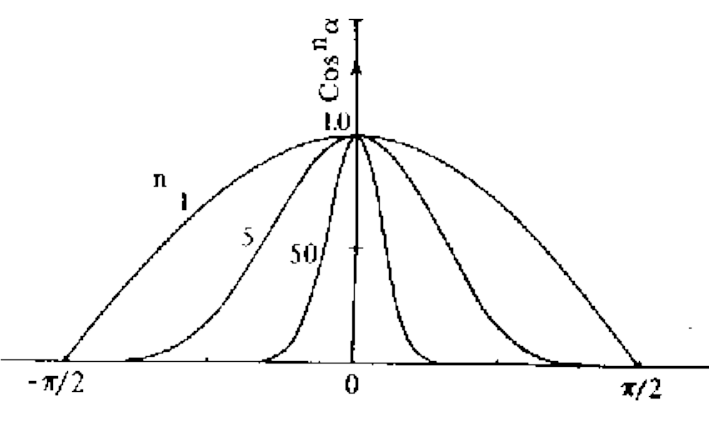
\includegraphics[width=60mm]{pics/cones_of_light.png}
	\caption{(a) shows an overview of how adjusting $\alpha$ changes the light cone of a simulated light source. (b) shows a modelled light cone, modelled with the shown measured light cone.\label{fig:cones_of_light}}
\end{figure}

\subsubsection{Modelling a reflection}
Light impinging on a surface can reflect in three different ways: Diffuse, spread and specular. Almost all surfaces combine several of these reflection types. A visualisation of these reflections can be seen in Figure \ref{fig:phong}.
\begin{figure}
	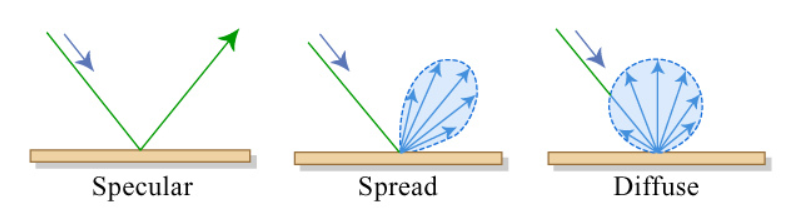
\includegraphics[width=\textwidth]{pics/3_reflections.png}
	\caption{The possible ways for light to reflect when it hits a surface \cite{3reflections}.\label{fig:phong}}
\end{figure}
The \textbf{specular reflection} is a so called perfect reflection. It reflects each incident ray outward, with the reflected ray having the same exit angle to the normal vector $N$ as the incident ray. A material with this kind of property is a mirror. The \textbf{diffuse reflection} is the opposite. Instead of reflecting light in one direction, the light ray is scattered in all directions following a Lambertian emission pattern. This leads to a point, which appears to have the same brightness, no matter the observation angle. A common material with this property is plain white paper. The final kind of reflection is the called the \textbf{spread reflection}. It's a scattered reflection, aimed in the direction of the ideal reflection. A material which has mainly this kind of reflection is matte aluminium.

All of these reflections can be modelled with the help of equation \ref{eq:Reflection}, where $\phi_2$ represents the observation angle. The first part of the equation calculates how much of the impinging light is reflected off the surface and not converted into heat. This is determined by $A$, which represent the albedo of the observed surface. 

The second part describes the actual reflection of the surface. $\frac{\alpha+1}{2\pi}\cos^\alpha(\theta_1'-\phi_2)$ describes the spread reflection and is modelled as light source pointing in the direction of the ideal reflection $\theta_1'$ (see equation \ref{eq:I(phi)}). The higher $\alpha$ is chosen, the more focused the reflection. If $\alpha$ is chosen to be infinite, the surface is modelled as a mirror instead.

$\frac{1}{\pi}\cos(\phi_2)$ describes the diffuse part of the equation and is also modelled with \ref{eq:I(phi)} where $\alpha = 1$. This results in a diffuse reflection. The final term of the equation is $r_d$. This value represents the ratio between the diffuse and spread reflection.

\begin{equation}
\label{eq:Reflection}
R(\theta_2) = E_{hor}\rho(\lambda)\left[ r_{d} \frac{1}{\pi}\cos(\phi_2)+ (1-r_{d})\frac{\alpha+1}{2\pi}\cos^\alpha(\theta_1'-\phi_2) \right]
\end{equation}

\subsubsection{Modelling a photo diode}
The final part missing in the model is the observer. The observer, or receiver in our case, is a photo diode which can be modelled with the help of Equation \ref{eq:receiver_PD}. This equation is very similar to equation \ref{eq:E_hor}, but has one major difference: The $rec(x)$ function. This function checks if the light incoming at angle $\theta_2$ lies in the field of view of the photo diode. If it is, then $rec \left(\frac{\theta_2}{FOV}\right)$ returns 1, otherwise it's 0 and the ray of light wont be counted.

\begin{equation}
	\label{eq:receiver_PD}
	PD = \frac{I\cos(\theta_2)}{d^2} rec \left(\frac{\theta_2}{FOV}\right)
	\qquad
	rec(x) = 
		\begin{cases}
		1, |x|\leq 1 \\
		0, |x| > 1 \\
		\end{cases}
\end{equation}

\subsubsection{Creating a 3D model}
All equations shown in the previous sections can be combined into one big equation, calculating how much a point on the wall is illuminated, reflected and perceived by the observer. This equation is \ref{eq:fullmodel}. It has however a lot of variables, which will make it hard to create a proper simulation. 

\begin{equation}
	\label{eq:fullmodel}
	PD_{tot} = I(\phi,\alpha_{light},\Phi_{lum}) R(\theta_1,\phi_2,\lambda,r_d,\alpha_{floor}) PD(\theta_2,d_2)
\end{equation}
This can be solved by making the problem concrete and simulate it in a 3D space with an $xyz$ coordinate system. If we assume the floor is a plane spanning x and y (thus z = 0) and fix the positions and normals of the LED and photo diode, we can express all angles and distances as formulas of x,y and z. If we then want to calculate total amount of energy perceived by the photo diode, all we need to do is integrate over all the points of the floor (the xy plane).
\begin{equation}
\label{eq:fullmodel_xy}
PD_{tot} = \int_x \int_y I(x,y,z,\alpha_{light},\Phi_{lum}) R(x,y,z,\lambda,r_d,\alpha_{floor}) PD(x,y,z)
\end{equation}

This model was used to create the model used in chapter \ref{Model}. That chapter will also explain what changes were made to obtain the presented model.